\section{三角函数}
\subsection{三角函数的概念}
\begin{figure}[ht]
	\centering
	\begin{tikzpicture}
		\draw[help lines, color=gray!30, dashed](0,0)grid(4,3);
		\coordinate(A)at(0,0);
		\coordinate(B)at(4,0);
		\coordinate(C)at(4,3);
		\draw (A)node[left]{\(A\)}
			--(B)node[right]{\(B\)}node[midway,below]{\(c\)}
			--(C)node[right]{\(C\)}node[midway,right]{\(a\)}
			--(A)node[midway,left,above]{\(b\)}
			pic["\(\theta\)",draw=orange,-,angle eccentricity=2,angle radius=0.3cm]{angle=B--A--C}
			pic[draw=gray,-,angle radius=0.3cm]{right angle=C--B--A};
	\end{tikzpicture}
	\caption{}
	\label{figure:函数.三角函数.三角函数的几何定义}
\end{figure}

\begin{definition}\label{definition:函数.三角函数的几何定义}
如\cref{figure:函数.三角函数.三角函数的几何定义},
取任意一个直角三角形\(\triangle ABC\),
其中\(\angle B\)是直角(即\(\angle ABC = \pi/2\)),
假设\(\angle BAC = \theta\).
定义三角函数如下:
\begin{center}
	\begin{tabular}{cc|cc|cc}
		\hline
		名称 & 定义式 & 名称 & 定义式 & 名称 & 定义式 \\ \hline
		正弦 & \(\sin\theta = a/b\)
			& 正切 & \(\tan\theta = a/c\)
				& 正割 & \(\sec\theta = b/c\) \\
		余弦 & \(\cos\theta = c/b\)
			& 余切 & \(\cot\theta = c/a\)
				& 余割 & \(\csc\theta = b/a\) \\
		\hline
	\end{tabular}
\end{center}
\end{definition}

\begin{example}
下面列出一些特殊的正弦函数值:\[
\sin0 = 0, \quad
\sin\frac{\pi}{6} = \frac{1}{2}, \quad
\sin\frac{\pi}{4} = \frac{\sqrt{2}}{2}, \quad
\sin\frac{\pi}{3} = \frac{\sqrt{3}}{2},
\]\[
\sin\frac{\pi}{2} = 1, \quad
\sin\pi = 0, \quad
\sin\frac{3\pi}{2} = -1.
\]

\begin{figure}[ht]
	\centering
	\begin{tikzpicture}
		\pgfmathsetmacro{\r}{2}
		\pgfmathsetmacro{\ax}{\r*cos(30)}
		\pgfmathsetmacro{\ay}{\r*sin(30)}
		\pgfmathsetmacro{\b}{\r/sqrt(2)}
		\coordinate (O)at(0,0);
		\draw(O)circle(\r);
		\begin{scope}[dashed,color=gray!50,text=black]
			\draw(O)--(\r,0)node[left]{\(0\)}node[right]{\(0\)}
			(O)--(\ax,\ay)node[below left]{\(\tfrac{\pi}{6}\)}node[right]{\(\tfrac{1}{2}\)}
			(O)--(\b,\b)node[below left]{\(\tfrac{\pi}{4}\)}node[above right]{\(\tfrac{\sqrt2}{2}\)}
			(O)--(\ay,\ax)node[below left]{\(\tfrac{\pi}{3}\)}node[above]{\(\tfrac{\sqrt3}{2}\)}
			(O)--(0,\r)node[below]{\(\tfrac{\pi}{2}\)}node[above]{\(1\)}
			(O)--(-\ay,\ax)node[below right]{\(\tfrac{2\pi}{3}\)}node[above]{\(\tfrac{\sqrt3}{2}\)}
			(O)--(-\b,\b)node[below right]{\(\tfrac{3\pi}{4}\)}node[above left]{\(\tfrac{\sqrt2}{2}\)}
			(O)--(-\ax,\ay)node[below right]{\(\tfrac{5\pi}{6}\)}node[left]{\(\tfrac{1}{2}\)}
			(O)--(-\r,0)node[right]{\(\pi\)}node[left]{\(0\)}
			(O)--(-\ax,-\ay)node[above right]{\(\tfrac{7\pi}{6}\)}node[left]{\(-\tfrac{1}{2}\)}
			(O)--(-\b,-\b)node[above right]{\(\tfrac{5\pi}{4}\)}node[below left]{\(-\tfrac{\sqrt2}{2}\)}
			(O)--(-\ay,-\ax)node[above right]{\(\tfrac{4\pi}{3}\)}node[below]{\(-\tfrac{\sqrt3}{2}\)}
			(O)--(0,-\r)node[above]{\(\tfrac{3\pi}{2}\)}node[below]{\(-1\)}
			(O)--(\ay,-\ax)node[above left]{\(\tfrac{5\pi}{3}\)}node[below]{\(-\tfrac{\sqrt3}{2}\)}
			(O)--(\b,-\b)node[above left]{\(\tfrac{7\pi}{4}\)}node[below right]{\(-\tfrac{\sqrt2}{2}\)}
			(O)--(\ax,-\ay)node[above left]{\(\tfrac{11\pi}{6}\)}node[right]{\(-\tfrac{1}{2}\)}
			;
		\end{scope}
		\begin{scope}[very thick,->]
			\draw(-1,0)--(1,0)node[above left]{\(x\)};
			\draw(0,-1)--(0,1)node[below right]{\(y\)};
		\end{scope}
	\end{tikzpicture}
	\caption{正弦函数\(\sin x\)的辅助圆与特殊值}
\end{figure}

特殊的余弦函数值:\[
	\cos0 = 1, \quad
	\cos\frac{\pi}{6} = \frac{\sqrt{3}}{2}, \quad
	\cos\frac{\pi}{4} = \frac{\sqrt{2}}{2}, \quad
	\cos\frac{\pi}{3} = \frac{1}{2},
\]\[
	\cos\frac{\pi}{2} = 0, \quad
	\cos\pi = -1, \quad
	\cos\frac{3\pi}{2} = 0.
\]
\end{example}

\subsection{三角函数的性质}
\begin{property}
根据三角函数的定义,显然有\begin{gather}
	\cot\theta = \frac{1}{\tan\theta}, \\
	\sec\theta = \frac{1}{\cos\theta}, \\
	\csc\theta = \frac{1}{\sin\theta}.
\end{gather}
\end{property}

\begin{theorem}[毕达哥拉斯三角恒等式]
\begin{figure}[ht]
	\def\subwidth{.5\linewidth}
	\def\subscale{.8}
		\begin{subfigure}[b]{\subwidth}%
		\centering
		\begin{tikzpicture}[scale=\subscale]
			\draw[help lines, color=gray!30, dashed] (0,0) grid (4,3);
			\coordinate (A) at (0,0);
			\coordinate (B) at (4,0);
			\coordinate (C) at (4,3);
			\draw (A)node[left]{\(A\)} -- (B)node[right]{\(B\)}node[midway,below]{\(\cos\theta\)} -- (C)node[right]{\(C\)}node[midway,right]{\(\sin\theta\)} -- (A)node[midway,above left]{\(1\)} pic["\(\theta\)",draw=orange,-,angle eccentricity=2,angle radius=0.3cm]{angle=B--A--C} pic[draw=gray,-,angle radius=0.3cm]{right angle=C--B--A};
		\end{tikzpicture}
		\subcaption{正弦、余弦辅助三角形}
		\end{subfigure}%
		\begin{subfigure}[b]{\subwidth}%
		\centering
		\begin{tikzpicture}[scale=\subscale]
			\draw[help lines, color=gray!30, dashed] (0,0) grid (4,3);
			\coordinate (A) at (0,0);
			\coordinate (B) at (4,0);
			\coordinate (C) at (4,3);
			\draw (A)node[left]{\(A\)} -- (B)node[right]{\(B\)}node[midway,below]{\(1\)} -- (C)node[right]{\(C\)}node[midway,right]{\(\tan\theta\)} -- (A)node[midway,above left]{\(\sec\theta\)} pic["\(\theta\)",draw=orange,-,angle eccentricity=2,angle radius=0.3cm]{angle=B--A--C} pic[draw=gray,-,angle radius=0.3cm]{right angle=C--B--A};
		\end{tikzpicture}
		\subcaption{正切、正割辅助三角形}
		\end{subfigure}%
	\caption{两种特殊的辅助三角形}
	\label{figure:函数.两种特殊的辅助三角形}
\end{figure}

结合\cref{figure:函数.两种特殊的辅助三角形},根据勾股定理可得
\begin{gather}
	\sin^2 \theta + \cos^2 \theta = 1,
		\label{equation:三角函数.毕达哥拉斯三角恒等式1} \\
	\tan^2 \theta + 1 = \sec^2 \theta, \\
	1 + \cot^2 \theta = \csc^2 \theta.
\end{gather}
\end{theorem}

\begin{figure}[ht]
	\centering
	\begin{tikzpicture}
		\pgfmathsetmacro{\a}{6}
		\coordinate(O)at(0,0);
		\pgfmathsetmacro{\t}{30}
		\draw(O)node[below left]{\(O\)}
			--(\a,0)coordinate(A)node[below right]{\(A\)}
			arc[start angle=0,end angle=\t,radius=\a]coordinate(B)node[right]{\(B\)}
			--(O);
		\draw(B)--(B|-A)coordinate(C)node[below right]{\(C\)};
		\draw(B)--(\a,{\a*tan(\t)})coordinate(D)node[above right]{\(D\)}--(\a,0);
		\pic["\(\theta\)",draw,-,angle eccentricity=1.5,angle radius=6mm]{angle=A--O--B};
		\begin{scope}[|<->|,black!40,every node/.style={black,midway,sloped}]
			\def\mark#1#2#3#4#5{%
				\draw($#1+#4$)--($#2+#4$)node[#3]{$#5$};%
			}%
			\mark{(C)}{(B)}{above}{(-5pt,0)}{\sin\theta}
			\mark{(O)}{(D)}{above}{({(-1em-10pt)*sin(30)},{(1em+10pt)*cos(30)})}{\sec\theta}
			\mark{(O)}{(B)}{above}{({-5pt*sin(30)},{5pt*cos(30)})}{1}
			\mark{(O)}{(C)}{below}{(0,-5pt)}{\cos\theta}
			\mark{(A)}{(D)}{below}{(5pt,0)}{\tan\theta}
			\mark{(O)}{(A)}{below}{(0,-1em-10pt)}{1}
		\end{scope}
	\end{tikzpicture}
	\caption{}
\end{figure}

\begin{figure}[ht]
	\centering
	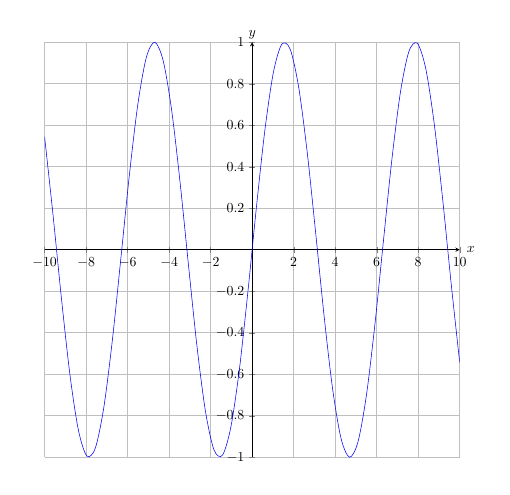
\begin{tikzpicture}[scale=.5]
		\begin{axis}[
			xmin=-10,xmax=10,
			restrict y to domain=-2:2,
			ymin=-1,ymax=1,
			grid=both,width=\textwidth,height=\textwidth,
			axis lines=middle,
			xlabel=$x$,
			ylabel=$y$,
			enlarge x limits=0.1,
			enlarge y limits=0.1,
			axis lines = middle,
			x label style={at={(ticklabel* cs:1.00)}, inner sep=5pt, anchor=west},
			y label style={at={(ticklabel* cs:1.00)}, inner sep=2pt, anchor=south},
		]
			\addplot[color=blue,samples=50,smooth,domain=-10:10,variable=\x]{sin(\x r)};
		\end{axis}
	\end{tikzpicture}
	\caption{正弦函数\(y=\sin x\)的图形}
	\label{figure:函数.正弦函数的图形}
\end{figure}

\begin{figure}
	\centering
	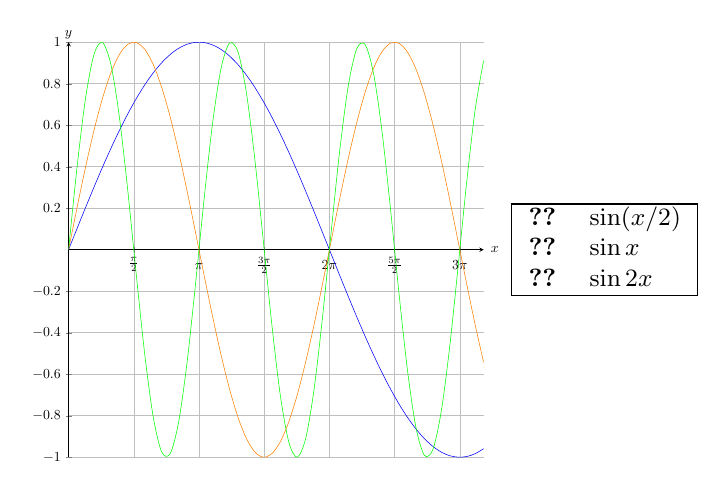
\begin{tikzpicture}[scale=.5]
		\begin{axis}[
			name=Sine,
			xmin=0,xmax=10,
			restrict y to domain=-2:2,
			ymin=-1,ymax=1,
			grid=both,width=\textwidth,height=\textwidth,
			axis lines=middle,
			xlabel=$x$,
			ylabel=$y$,
			axis lines = middle,
			x label style={at={(ticklabel* cs:1.00)}, inner sep=5pt, anchor=west},
			y label style={at={(ticklabel* cs:1.00)}, inner sep=2pt, anchor=south},
			xtick={0,1.5708,3.1416,...,10},
			xticklabels={
				$\relax$,
				$\frac{\pi}{2}$,
				$\pi\vphantom{\frac12}$,
				$\frac{3\pi}{2}$,
				$2\pi\vphantom{\frac12}$,
				$\frac{5\pi}{2}$,
				$3\pi\vphantom{\frac12}$,
			},
		]
			\addplot[color=blue,samples=50,smooth,domain=0:10,variable=\x]
				{sin(.5*\x r)};\label{pgfplots:正弦函数.sin(x/2)}
			\addplot[color=orange,samples=50,smooth,domain=0:10,variable=\x]
				{sin(\x r)};\label{pgfplots:正弦函数.sin(x)}
			\addplot[color=green,samples=50,smooth,domain=0:10,variable=\x]
				{sin(2*\x r)};\label{pgfplots:正弦函数.sin(2*x)}
		\end{axis}
		\node[draw,fill=white,inner sep=0pt,right=1em]at(Sine.east){\small\begin{tabular}{cl}
		\ref{pgfplots:正弦函数.sin(x/2)} & \(\sin(x/2)\) \\
		\ref{pgfplots:正弦函数.sin(x)} & \(\sin x\) \\
		\ref{pgfplots:正弦函数.sin(2*x)} & \(\sin2x\) \\
		\end{tabular}};
	\end{tikzpicture}
	\caption{}
\end{figure}

\begin{property}
如\cref{figure:函数.正弦函数的图形},
可以观察得出正弦函数的若干性质.
\begin{enumerate}
	\item 正弦函数是周期函数,其周期为\(T = 2\pi\).
	\item 正弦函数在区间\([2k\pi-\frac{\pi}{2},2k\pi+\frac{\pi}{2})\)上单调递增.
	\item 在区间\([2k\pi+\frac{\pi}{2},2k\pi+\frac{3\pi}{2})\)上单调递增.
	\item 当\(x=\frac{\pi}{2}+2k\pi\ (k\in\mathbb{Z})\)时,正弦函数\(y=\sin x\)取得极大值\(1\).
	\item 当\(x=\frac{3\pi}{2}+2k\pi\ (k\in\mathbb{Z})\)时,正弦函数\(y=\sin x\)取得极小值\(-1\).
	\item 正弦函数是奇函数,其图形关于坐标原点\(O\)中心对称,满足\(\sin(-x)=-\sin x\).
\end{enumerate}
\end{property}

\begin{figure}[ht]
	\centering
	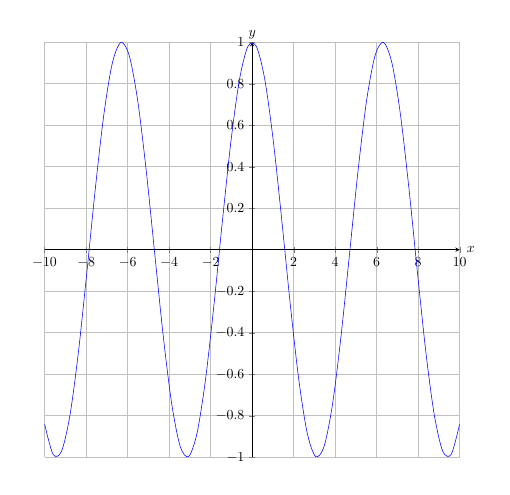
\begin{tikzpicture}[scale=.5]
		\begin{axis}[
			xmin=-10,xmax=10,
			restrict y to domain=-2:2,
			ymin=-1,ymax=1,
			grid=both,width=\textwidth,height=\textwidth,
			axis lines=middle,
			xlabel=$x$,
			ylabel=$y$,
			enlarge x limits=0.1,
			enlarge y limits=0.1,
			axis lines = middle,
			x label style={at={(ticklabel* cs:1.00)}, inner sep=5pt, anchor=west},
			y label style={at={(ticklabel* cs:1.00)}, inner sep=2pt, anchor=south},
		]
			\addplot[color=blue,samples=50,smooth,domain=-10:10,variable=\x]{cos(\x r)};
		\end{axis}
	\end{tikzpicture}
	\caption{余弦函数\(y=\cos x\)的图形}
	\label{figure:函数.余弦函数的图形}
\end{figure}

\begin{figure}
	\centering
	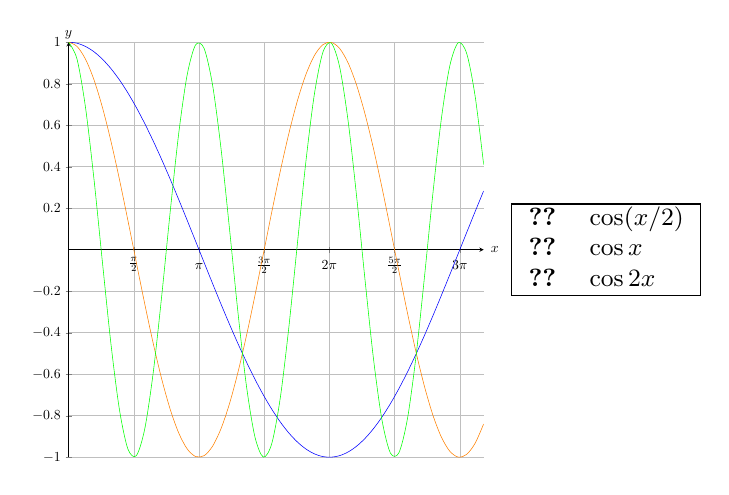
\begin{tikzpicture}[scale=.5]
		\begin{axis}[
			name=Cosine,
			xmin=0,xmax=10,
			restrict y to domain=-2:2,
			ymin=-1,ymax=1,
			grid=both,width=\textwidth,height=\textwidth,
			axis lines=middle,
			xlabel=$x$,
			ylabel=$y$,
			axis lines = middle,
			x label style={at={(ticklabel* cs:1.00)}, inner sep=5pt, anchor=west},
			y label style={at={(ticklabel* cs:1.00)}, inner sep=2pt, anchor=south},
			xtick={0,1.5708,3.1416,...,10},
			xticklabels={
				$\relax$,
				$\frac{\pi}{2}$,
				$\pi\vphantom{\frac12}$,
				$\frac{3\pi}{2}$,
				$2\pi\vphantom{\frac12}$,
				$\frac{5\pi}{2}$,
				$3\pi\vphantom{\frac12}$,
			},
		]
			\addplot[color=blue,samples=50,smooth,domain=0:10,variable=\x]
				{cos(.5*\x r)};\label{pgfplots:余弦函数.cos(x/2)}
			\addplot[color=orange,samples=50,smooth,domain=0:10,variable=\x]
				{cos(\x r)};\label{pgfplots:余弦函数.cos(x)}
			\addplot[color=green,samples=50,smooth,domain=0:10,variable=\x]
				{cos(2*\x r)};\label{pgfplots:余弦函数.cos(2*x)}
		\end{axis}
		\node[draw,fill=white,inner sep=0pt,right=1em]at(Cosine.east){\small\begin{tabular}{cl}
		\ref{pgfplots:余弦函数.cos(x/2)} & \(\cos(x/2)\) \\
		\ref{pgfplots:余弦函数.cos(x)} & \(\cos x\) \\
		\ref{pgfplots:余弦函数.cos(2*x)} & \(\cos2x\) \\
		\end{tabular}};
	\end{tikzpicture}
	\caption{}
\end{figure}

\begin{property}
如\cref{figure:函数.余弦函数的图形},
可以观察得出余弦函数的若干性质.
\begin{enumerate}
	\item 余弦函数也是周期函数,其周期为\(T = 2\pi\).
	\item 余弦函数在区间\([2k\pi,\pi+2k\pi)\)上单调递减.
	\item 在区间\([\pi+2k\pi,2\pi+2k\pi)\)上单调递增.
	\item 当\(x=2k\pi\ (k\in\mathbb{Z})\)时,余弦函数\(y=\cos x\)取得极大值\(1\).
	\item 当\(x=(2k-1)\pi\ (k\in\mathbb{Z})\)时,余弦函数\(y=\cos x\)取得极小值\(-1\).
	\item 余弦函数是偶函数,其图形关于\(y\)轴对称,满足\(\cos(-x)=\cos x\).
\end{enumerate}
\end{property}

\begin{figure}[ht]
	\centering
	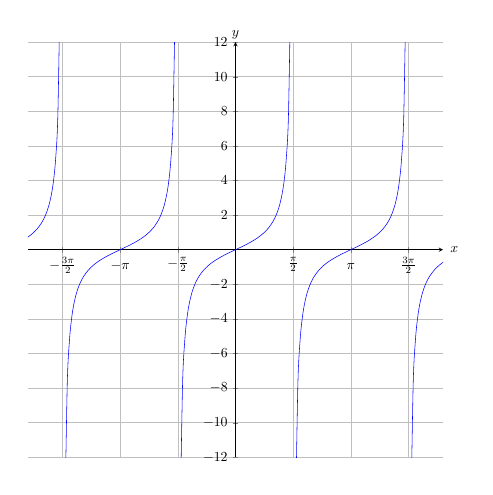
\begin{tikzpicture}[scale=.5]
		\begin{axis}[
			restrict y to domain=-20:20,
			ymin=-10,ymax=10,
			grid=both,width=\textwidth,height=\textwidth,
			axis lines=middle,
			xlabel=$x$,
			ylabel=$y$,
			enlarge x limits=0.1,
			enlarge y limits=0.1,
			x label style={at={(ticklabel* cs:1.00)}, inner sep=5pt, anchor=west},
			y label style={at={(ticklabel* cs:1.00)}, inner sep=2pt, anchor=south},
			xmin=-4.7124, xmax=4.7124,
			xtick={-4.7124,-3.1416,-1.5708,...,10},
			xticklabels={
				$-\frac{3\pi}{2}$,
				$-\pi\vphantom{\frac{1}{2}}$,
				$-\frac{\pi}{2}$,
				$\relax$,%不能去掉\relax
				$\frac{\pi}{2}$,
				$\pi\vphantom{\frac{1}{2}}$,
				$\frac{3\pi}{2}$,
			},
		]
			\foreach \i in {-5,-3,...,3} {
				\addplot[color=blue,samples=50,smooth,domain={\i*pi/2}:{(\i+2)*pi/2},variable=\x]
				{tan(\x r)};
			}
		\end{axis}
	\end{tikzpicture}
	\caption{正切函数\(y=\tan x\)的图形}
	\label{figure:函数.正切函数的图形}
\end{figure}

\begin{property}
如\cref{figure:函数.正切函数的图形},
可以观察得出正切函数的若干性质.
\begin{enumerate}
	\item 正切函数是周期函数,其周期为\(T = \pi\).
	\item 正切函数在区间\((k\pi-\frac{\pi}{2},k\pi+\frac{\pi}{2})\ (k\in\mathbb{Z})\)上单调递增.
	\item 正切函数是奇函数,其图形关于坐标原点\(O\)中心对称,满足\(\tan(-x)=-\tan x\).
\end{enumerate}
\end{property}

\begin{figure}[ht]
	\centering
	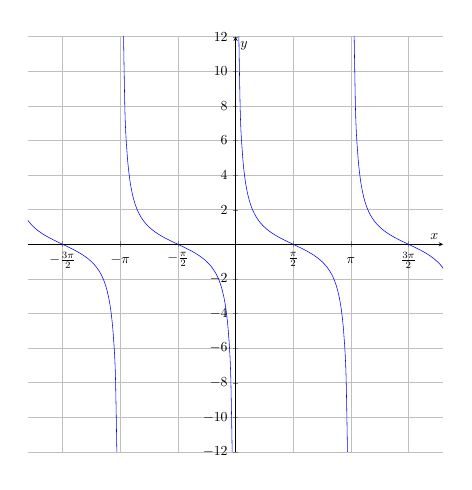
\begin{tikzpicture}[scale=.5]
		\begin{axis}[
			restrict y to domain=-20:20,
			ymin=-10,ymax=10,
			grid=both,width=\textwidth,height=\textwidth,
			axis lines=middle,
			xlabel=$x$,
			ylabel=$y$,
			enlarge x limits=0.1,
			enlarge y limits=0.1,
			xmin=-4.7124, xmax=4.7124,
			xtick={-4.7124,-3.1416,-1.5708,...,10},
			xticklabels={
				$-\frac{3\pi}{2}$,
				$-\pi\vphantom{\frac{1}{2}}$,
				$-\frac{\pi}{2}$,
				$\relax$,%不能去掉\relax
				$\frac{\pi}{2}$,
				$\pi\vphantom{\frac{1}{2}}$,
				$\frac{3\pi}{2}$,
			},
		]
		\foreach \i in {-2,-1,0,1} {
			\addplot[color=blue,samples=50,smooth,domain={\i*pi}:{(\i+1)*pi},variable=\x]
			{cot(\x r)};
		}
		\end{axis}
	\end{tikzpicture}
	\caption{余切函数\(y=\cot x\)的图形}
\end{figure}

\subsection{和积互化公式}
\begin{theorem}[和积互化公式]
设\(\alpha,\beta\in\mathbb{R}\),则有
\begin{gather}
	\sin(\alpha\pm\beta) = \sin\alpha\cos\beta\pm\cos\alpha\sin\beta,
	\label{equation:函数.三角函数.和积互化公式1} \\
	\cos(\alpha\pm\beta) = \cos\alpha\cos\beta\mp\sin\alpha\sin\beta,
	\label{equation:函数.三角函数.和积互化公式2} \\
	\tan(\alpha\pm\beta) = \frac{\tan\alpha\pm\tan\beta}{1\mp\tan\alpha\tan\beta},
	\label{equation:函数.三角函数.和积互化公式3} \\
	\cot(\alpha\pm\beta) = \frac{\cot\alpha\cot\beta\mp 1}{\cot\beta\pm\cot\alpha},
	\label{equation:函数.三角函数.和积互化公式4} \\
	\sec(\alpha\pm\beta) = \frac{\sec\alpha\sec\beta}{1\mp\tan\alpha\tan\beta},
	\label{equation:函数.三角函数.和积互化公式5} \\
	\csc(\alpha\pm\beta) = \frac{\csc\alpha\csc\beta}{\cot\beta\pm\cot\alpha},
	\label{equation:函数.三角函数.和积互化公式6} \\
	\sin \alpha \cos \beta = \frac{\sin (\alpha + \beta) + \sin (\alpha - \beta)}{2},
	\label{equation:函数.三角函数.和积互化公式7} \\
	\cos \alpha \sin \beta = \frac{\sin (\alpha + \beta) - \sin (\alpha - \beta)}{2},
	\label{equation:函数.三角函数.和积互化公式8} \\
	\cos \alpha \cos \beta = \frac{\cos (\alpha + \beta) + \cos (\alpha - \beta)}{2},
	\label{equation:函数.三角函数.和积互化公式9} \\
	\sin \alpha \sin \beta = -\frac{\cos (\alpha + \beta) - \cos (\alpha - \beta)}{2},
	\label{equation:函数.三角函数.和积互化公式10} \\
	\sin \alpha + \sin \beta = 2 \sin \frac{\alpha + \beta}{2} \cos \frac{\alpha - \beta}{2},
	\label{equation:函数.三角函数.和积互化公式11} \\
	\sin \alpha - \sin \beta = 2 \cos \frac{\alpha + \beta}{2} \sin \frac{\alpha - \beta}{2},
	\label{equation:函数.三角函数.和积互化公式12} \\
	\cos \alpha + \cos \beta = 2 \cos \frac{\alpha + \beta}{2} \cos \frac{\alpha - \beta}{2},
	\label{equation:函数.三角函数.和积互化公式13} \\
	\cos \alpha - \cos \beta = -2 \sin \frac{\alpha + \beta}{2} \sin \frac{\alpha - \beta}{2}.
	\label{equation:函数.三角函数.和积互化公式14}
\end{gather}
\begin{proof}
\begin{figure}[ht]
	\centering
	\begin{tikzpicture}
		\coordinate(A)at(0.0,0.0);
		\coordinate(B)at(6.4,0.0);
		\coordinate(C)at(6.4,4.8);
		\coordinate(D)at(6.4,6.4);
		\coordinate(E)at(5.2,6.4);
		\draw (A)
			--(B)node[midway,below]{\(\cos\alpha\cos\beta\)}
			--(C)node[midway,right]{\rotatebox{90}{\(\cos\alpha\sin\beta\)}}
			--(D)node[midway,right]{\rotatebox{90}{\(\sin\alpha\cos\beta\)}}
			--(E)node[midway,above]{\(\sin\alpha\sin\beta\)}
			--(C)node[midway,left=2mm,below=-3mm]{\rotatebox{-53.13}{\(\sin\alpha\)}}
			--(A)node[midway,right=1mm,below=-2mm]{\rotatebox{36.87}{\(\cos\alpha\)}}
			--(E)node[midway,left=2mm,above=2mm]{\(1\)};
		\pic["\(\alpha\)",draw=orange,-,angle eccentricity=2,angle radius=0.7cm]{angle=C--A--E};
		\pic["\(\beta\)",draw=blue,-,angle eccentricity=2,angle radius=0.7cm]{angle=B--A--C};
		\pic[draw=blue,-,angle radius=0.5cm]{angle=D--C--E};
		\pic[draw=gray,-,angle radius=0.3cm]{right angle=C--B--A};
		\pic[draw=gray,-,angle radius=0.3cm]{right angle=E--C--A};
		\pic[draw=gray,-,angle radius=0.3cm]{right angle=E--D--C};
	\end{tikzpicture}
	\caption{和积互化公式的辅助三角形}
	\label{figure:函数.和积互化公式的辅助三角形}
\end{figure} %

观察\cref{figure:函数.和积互化公式的辅助三角形} 可知
\begin{align*}
	\sin(\alpha+\beta) &= \sin\alpha\cos\beta+\cos\alpha\sin\beta, \\
	\cos(\alpha+\beta) &= \cos\alpha\cos\beta-\sin\alpha\sin\beta
\end{align*}成立.
又令\(\beta=-\beta\)则可得
\begin{align*}
	\sin(\alpha-\beta) &= \sin\alpha\cos\beta-\cos\alpha\sin\beta, \\
	\cos(\alpha-\beta) &= \cos\alpha\cos\beta+\sin\alpha\sin\beta.
	\qedhere
\end{align*}
\end{proof}
\end{theorem}

特别地,根据和积互化公式有
\begin{gather}
	\sin(\pi+\alpha) = -\sin\alpha, \\
	\cos(\pi+\alpha) = -\cos\alpha, \\
	\tan(\pi+\alpha) = \tan\alpha, \\
	\cot(\pi+\alpha) = \cot\alpha, \\
	\sin(\pi-\alpha) = \sin\alpha, \\
	\cos(\pi-\alpha) = -\cos\alpha, \\
	\tan(\pi-\alpha) = -\tan\alpha, \\
	\cot(\pi-\alpha) = -\cot\alpha.
\end{gather}
还有
\begin{gather}
	\cos\left(\frac{\pi}{2}-\alpha\right) = \sin\alpha, \\
	\sin\left(\frac{\pi}{2}-\alpha\right) = \cos\alpha, \\
	\tan\left(\frac{\pi}{2}-\alpha\right) = \cot\alpha, \\
	\cot\left(\frac{\pi}{2}-\alpha\right) = \tan\alpha.
\end{gather}
以上四个公式是当\(\alpha\)为任意角时
\(\left(\frac{\pi}{2}-\alpha\right)\)的诱导公式.
如果把其中的\(\alpha\)换成\((-\alpha)\),
就可得到当\(\alpha\)为任意角时
\(\left(\frac{\pi}{2}+\alpha\right)\)的诱导公式:
\begin{gather}
	\cos\left(\frac{\pi}{2}+\alpha\right) = -\sin\alpha, \\
	\sin\left(\frac{\pi}{2}+\alpha\right) = \cos\alpha, \\
	\tan\left(\frac{\pi}{2}+\alpha\right) = -\cot\alpha, \\
	\cot\left(\frac{\pi}{2}+\alpha\right) = -\tan\alpha.
\end{gather}

%\begin{example}
%\def\s{\sum\limits_{k=1}^n}%
%证明:
%当\(x\neq0\)时,有
%\begin{gather}
%	\s \sin kx
%	= \frac{\sin\frac{nx}{2} \sin\frac{(n+1)x}{2}}{\sin\frac{x}{2}}, \\
%	\s \cos kx
%	= \frac{\sin\frac{nx}{2} \cos\frac{(n+1)x}{2}}{\sin\frac{x}{2}}.
%\end{gather}
%TODO
%\end{example}

\subsection{倍角公式}
\begin{proposition}[二倍角公式]
设\(\alpha\in\mathbb{R}\),则有
\begin{align}
	\sin2\alpha &= 2 \sin\alpha \cos\alpha,
		\label{equation:三角函数.正弦的二倍角公式} \\
	\cos2\alpha &= \cos^2\alpha - \sin^2\alpha
		\label{equation:三角函数.余弦的二倍角公式1} \\
		&= 2 \cos^2\alpha - 1 \\
		&= 1 - 2 \sin^2\alpha, \\
	\tan2\alpha &= \frac{2 \tan\alpha}{1 - \tan^2\alpha}.
		\label{equation:三角函数.正切的二倍角公式}
\end{align}
\begin{proof}
在\cref{equation:函数.三角函数.和积互化公式1,equation:函数.三角函数.和积互化公式2} 中,
令\(\beta=\alpha\),就有\[
	\sin2\alpha
	=\sin(\alpha+\alpha)
	=\sin\alpha\cos\alpha+\cos\alpha\sin\alpha
	=2\sin\alpha\cos\alpha,
	\eqno(1)
\]\[
	\cos2\alpha
	=\cos(\alpha+\alpha)
	=\cos\alpha\cos\alpha-\sin\alpha\sin\alpha
	=\cos^2\alpha-\sin^2\alpha.
	\eqno(2)
\]
考虑到\cref{equation:三角函数.毕达哥拉斯三角恒等式1},
\(\sin^2\alpha+\cos^2\alpha=1\),
于是(2)又可以化为以下两种形式:\[
	\cos2\alpha
	=(\cos^2\alpha-\sin^2\alpha)+(1-\sin^2\alpha-\cos^2\alpha)
	=1-2\sin^2\alpha,
\]\[
	\cos2\alpha
	=(\cos^2\alpha-\sin^2\alpha)+(\sin^2\alpha+\cos^2\alpha-1)
	=2\cos^2\alpha-1.
\]
接着只需要将(1)式与(2)式等号两边分别相除,得\[
	\tan2\alpha=\frac{\sin2\alpha}{\cos2\alpha}
	=\frac{2\sin\alpha\cos\alpha}{cos^2\alpha-\sin^2\alpha}
	=\frac{\frac{2\sin\alpha\cos\alpha}{\cos^2\alpha}}{\frac{cos^2\alpha-\sin^2\alpha}{\cos^2\alpha}}
	=\frac{2\tan\alpha}{1-\tan^2\alpha}.
	\qedhere
\]
\end{proof}
\end{proposition}

\begin{proposition}[半倍角公式]
\begin{align}
	\sin \frac{\alpha}{2} &= \pm \sqrt{\frac{1 - \cos\alpha}{2}}, \\
	\cos \frac{\alpha}{2} &= \pm \sqrt{\frac{1 + \cos\alpha}{2}}, \\
	\tan \frac{\alpha}{2}
	&= \frac{\sin\alpha}{1+\cos\alpha} \\
	&= \frac{1-\cos\alpha}{\sin\alpha} \\
	&= \pm \sqrt{\frac{1 - \cos\alpha}{1 + \cos\alpha}}.
\end{align}
\begin{proof}
联立\[
	\left\{ \begin{array}{l}
		\cos^2\alpha - \sin^2\alpha = \cos 2\alpha, \\
		\cos^2\alpha + \sin^2\alpha = 1,
	\end{array} \right.
\]
整理得\[
	2\cos^2\alpha=1+\cos2\alpha, \qquad
	2\sin^2\alpha=1-\cos2\alpha,
\]
即\[
	\cos^2\alpha=\frac{1+\cos2\alpha}{2}, \qquad
	\sin^2\alpha=\frac{1-\cos2\alpha}{2},
\]
在等号两边同时开方,得\[
	\cos\alpha = \pm\sqrt{\frac{1+\cos2\alpha}{2}}, \qquad
	\sin\alpha = \pm\sqrt{\frac{1-\cos2\alpha}{2}},
\]
再相除可得\[
	\tan\alpha = \frac{\sin\alpha}{\cos\alpha}
	= \pm \sqrt{\frac{1 - \cos2\alpha}{1 + \cos2\alpha}}.
	\qedhere
\]
\end{proof}
\end{proposition}

\begin{figure}[ht]
	\centering
	\begin{tikzpicture}[scale=4]
		\pgfmathsetmacro{\t}{60}
		\coordinate(C)at({cos(\t)},{sin(\t)});
		\draw(1,0)coordinate(A)node[right]{\(A\)}
			arc[start angle=0,end angle=180,radius=1]
			coordinate(B)node[left]{\(B\)}--(0,0)coordinate(O)node[below]{\(O\)}
			--(C)node[above right]{\(C\)};
		\draw(C)--(C|-A)coordinate(D)node[below]{\(D\)}
			node[midway,above,rotate=90,orange]{\(\sin\theta\)};
		\draw(O)--(D)node[midway,below,orange]{\(\cos\theta\)}
			--(A)node[midway,below,orange]{\(1-\cos\theta\)}
			--(C)--(B)--(O)node[midway,below,orange]{\(1\)}
			pic[draw=gray,angle radius=0.3cm]{right angle=A--D--C}
			pic[draw=gray,angle radius=0.3cm]{right angle=B--C--A}
			pic["$\frac{\theta}{2}$",draw=cyan,angle eccentricity=1.7,angle radius=5mm]{angle=D--C--A}
			pic["$\frac{\theta}{2}$",draw=cyan,angle eccentricity=1.7,angle radius=5mm]{angle=A--B--C}
			pic["$\theta$",draw=blue,angle eccentricity=1.7,angle radius=5mm]{angle=D--O--C};
	\end{tikzpicture}
	\caption{半角公式的辅助三角形}
	\label{figure:函数.半角公式的辅助三角形}
\end{figure}

\begin{proposition}[万能公式]
\def\HalfAlpha{\frac\alpha2}
设\(\alpha\in\mathbb{R}\),则有
\begin{gather}
	\sin\alpha = \frac{2 \tan\HalfAlpha}{1+\tan^2\HalfAlpha},
		\label{equation:三角函数.万能公式1} \\
	\cos\alpha = \frac{1-\tan^2\HalfAlpha}{1+\tan^2\HalfAlpha},
		\label{equation:三角函数.万能公式2} \\
	\tan\alpha = \frac{2 \tan\HalfAlpha}{1-\tan^2\HalfAlpha}.
		\label{equation:三角函数.万能公式3}
\end{gather}
\begin{proof}
由\cref{equation:三角函数.正切的二倍角公式} 立即可得\[
	\tan\alpha
	=\frac{2\tan\HalfAlpha}{1-\tan^2\HalfAlpha}.
\]
由\cref{equation:三角函数.正弦的二倍角公式,equation:三角函数.余弦的二倍角公式1} 可得\[
	\sin\alpha
	=2\sin\HalfAlpha\cos\HalfAlpha
	=\frac{2\sin\HalfAlpha\cos\HalfAlpha}{\cos^2\HalfAlpha+\sin^2\HalfAlpha}
	=\frac{2\tan^2\HalfAlpha}{1+\tan^2\HalfAlpha},
\]\[
	\cos\alpha
	=\cos^2\HalfAlpha-\sin^2\HalfAlpha
	=\frac{\cos^2\HalfAlpha-\sin^2\HalfAlpha}{\cos^2\HalfAlpha+\sin^2\HalfAlpha}
	=\frac{1-\tan^2\HalfAlpha}{1+\tan^2\HalfAlpha}.
	\qedhere
\]
\end{proof}
\end{proposition}

\subsection{辅助角公式}
\begin{proposition}[辅助角公式]
设\(x\in\mathbb{R}\),
\(a,b\in\mathbb{R}^*\),
总有
\begin{equation}
	a \sin x + b \cos x = \sqrt{a^2 + b^2} \sin(x + \phi),
\end{equation}
其中\(\phi = \arctan\frac{b}{a}\).
\begin{proof}
令\(a = c \cos\phi,
b = c \sin\phi\ (c>0)\),那么
\[
	\left(a/c\right)^2+\left(b/c\right)^2
	=\cos^2\phi+\sin^2\phi
	=1
	\implies
	c = \sqrt{a^2+b^2};
\]
且\[
	\frac{b}{a} = \frac{c \sin\phi}{c \cos\phi} = \tan\phi
	\implies
	\phi = \arctan\frac{b}{a};
\]
同时
\[
	a \sin x + b \cos x
	= c (\sin x \cos\phi + \cos x \sin\phi)
	= c \sin(x+\phi).
	\qedhere
\]
\end{proof}
\end{proposition}

\subsection{正(余)弦函数的一般形式}
\begin{definition}
一般地,把函数\[
F(t) = A \sin(\omega t + \phi) \quad (-\infty<t<+\infty)
\]称作正弦函数的一般形式,其中\(A\)称为\DefineConcept{振幅},\(\omega\)称为\DefineConcept{角速度},\(\phi\)称为\DefineConcept{初相},\((\omega t + \phi)\)称为\DefineConcept{相位},\(T = \frac{2\pi}{\omega}\)称为\DefineConcept{最小正周期},\(f = \frac{1}{T}\)称为\DefineConcept{频率}.
\end{definition}
% Mathematica: Manipulate[Plot[A Sin[\[Omega] x + \[Phi]], {x, 0, 2 \[Pi]}], {A, 1, 5, 1}, {\[Omega], .1, 2, .1}, {\[Phi], 0, 2 \[Pi], \[Pi]/10}]
可以证明,随着\(A\)的增大,函数\(F(t)\)的波峰(或波谷)会变得更高(或更低);而随着\(\omega\)的增大,在固定长度的区间\([0,2\pi]\)上函数\(F(t)\)出现零点的次数会变多,形象地说,就是函数\(F(t)\)的图形变密了;另外,随着\(\phi\)的增大,看起来,函数\(f(t)\)的图形好像沿着\(x\)轴向左移动一样.
